%
% geradeapp.tex
%
% (c) 2018 Prof Dr Andreas Müller, Hochschule Rapperswil
%
\documentclass[tikz]{standalone}
\usepackage{times}
\usepackage{amsmath}
\usepackage{txfonts}
\usepackage[utf8]{inputenc}
\usepackage{graphics}
\usepackage{color}
\usepackage{pifont}
\usetikzlibrary{arrows,intersections,math,calc}
\begin{document}

\def\punkt#1{
        \fill[color=white] #1 circle[radius=0.08];
        \draw #1 circle[radius=0.08];
}

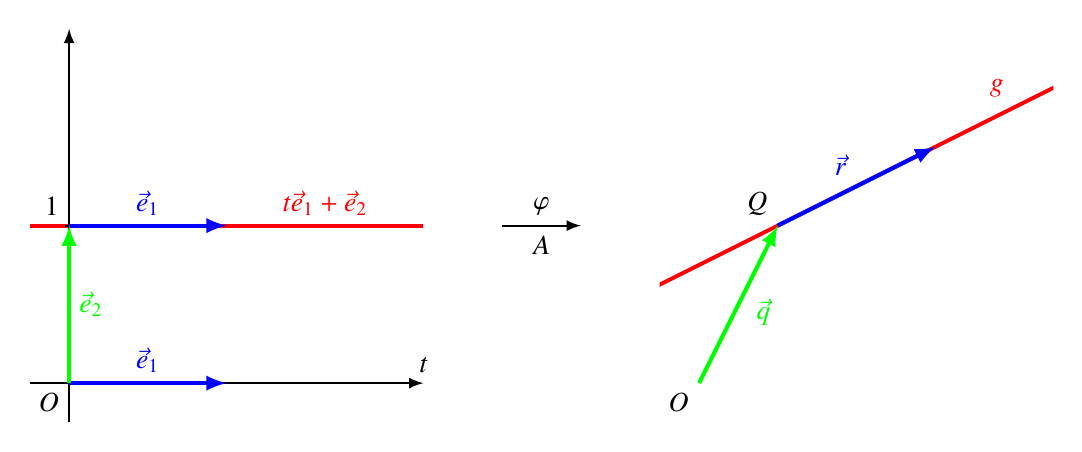
\begin{tikzpicture}[>=latex,thick]

% originalbild
\begin{scope}[xshift=-4cm]
\draw[color=red,line width=1.5pt] (-0.5,2)--(4.5,2);
\draw[->] (-0.5,0)--(4.5,0) coordinate[label=$t$];
\draw[->] (0,-0.5)--(0,4.5);
\draw (-0.05,2)--(0.05,2);
\node at (0,2) [above left] {$1$};
\node at (0,0) [below left] {$O$};

\draw[->,color=blue,line width=1.5pt] (0,0)--(2,0);
\node[color=blue]  at (1,0) [above] {$\vec{e}_1$};
\draw[->,color=blue,line width=1.5pt] (0,2)--(2,2);
\node[color=blue]  at (1,2) [above] {$\vec{e}_1$};

\draw[->,color=green,line width=1.5pt] (0,0)--(0,2);
\node[color=green] at (0,1) [right] {$\vec{e}_2$};

\node[color=red] at (3.25,2) [above] {$t\vec{e}_1+\vec{e}_2$};

\punkt{(0,0)}
\end{scope}

% Pfeil
\draw[->] (1.5,2)--(2.5,2);
\node at (2,2) [above] {$\varphi$};
\node at (2,2) [below] {$A$};

% affines Bild
\begin{scope}[xshift=4cm]
\coordinate (P0) at (1,2);
\coordinate (R) at (2,1);
\begin{scope}
\clip (-0.5,-0.5) rectangle (4.5,4.5);
\draw[color=red,line width=1.4pt] ($(P0)-3*(R)$)--($(P0)+3*(R)$);
\end{scope}

\draw[->,line width=1.5pt,color=green] (0,0)--(P0);
\node[color=green] at ($0.6*(P0)$) [below right] {$\vec{q}$};

\draw[->,line width=1.5pt,color=blue] (P0)--($(P0)+(R)$);
\node[color=blue] at ($(P0)+0.5*(R)$) [above left] {$\vec{r}$};

\punkt{(0,0)}
\node at (0,0) [below left] {$O$};

\node[color=red] at ($(P0)+1.5*(R)$) [above left] {$g$};

\punkt{(P0)}
\node at (P0) [above left] {$Q$};

\end{scope}

\end{tikzpicture}

\end{document}

